\documentclass{beamer}
\usepackage{amssymb,latexsym,amssymb,amsmath,amsbsy,amsopn,amstext,upgreek}
\usepackage{color,multicol}
\usepackage{graphicx,wrapfig,fancybox,watermark,graphics}
\usepackage{picins}
\usepackage{pgf}
\usepackage{media9}
\usepackage{hyperref}
\hypersetup{
    pdfpagemode=FullScreen, % show in full screen?
}
\usepackage{pdfpages}

\usepackage{listings,bera}
\definecolor{keywords}{RGB}{255,0,90}
\definecolor{comments}{RGB}{60,179,113}
\lstset{language=C,
    keywordstyle=\color{keywords},
    commentstyle=\color{comments}\emph
}
\usepackage{algorithm}
\usepackage{algorithmic}
\renewcommand{\algorithmicrequire}{\textbf{Input:}}
\renewcommand{\algorithmicensure}{\textbf{Output:}}

% reference entry
\usepackage{bibentry}
\usepackage[numbers]{natbib}

\usepackage[
    compress,
    %minimal,
    nonav,
    red,
    %gold,
    %blue,
    %numbers,
    %nologo,
    polyu,
    comp,
    %forty,
]
{beamerthemeHongKong}

\begin{document}

\title[Title short]{Title full}
\author[Author short]{Author full}
\institute[institute]{institute full name}
\date{\today}
\frame{\titlepage}


\section*{Table of Contents}
\frame {
  \frametitle{\secname}
  \tableofcontents
}

\AtBeginSubsection[] {
  \frame<handout:0> {
    \frametitle{Outline}
    \tableofcontents[current,currentsubsection]
  }
}

\section{Section A}

\subsection{Subsection A-A}

\begin{frame}
\frametitle{\subsecname}
  \begin{columns}
  \column{0.5\textwidth}
    \begin{figure}
    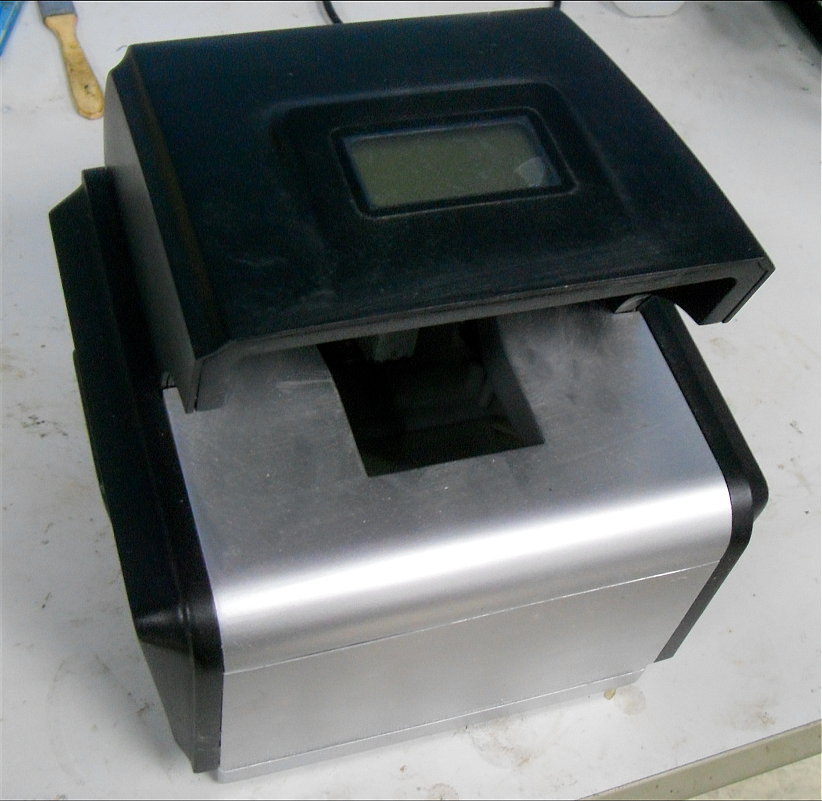
\includegraphics[width=\textwidth]{image/test-image1}
    \caption{figure A}
    \end{figure}
  \column{0.5\textwidth}
    \begin{block}{example}
      \begin{enumerate}
        \item<alert@1>
        text about figure A
        \item
        text
      \end{enumerate}
    \end{block}
  \end{columns}
\end{frame}

\subsection{Subsection A-B}

\section{Section B}

\section{Section C}

\subsection*{Thanks}

\begin{frame}
\frametitle{\subsecname}
  \begin{columns}
  \column{2.5cm}
  \column{5cm}
    \Huge{Thank you!}
  \column{2.5cm}
  \end{columns}
\end{frame}


\end{document}
